\documentclass[11pt]{article}

\usepackage[utf8]{inputenc} % character encoding - you don't need to understand this

% below are a bunch of useful packages, it doesn't cost anything to include them all so you might as well
\usepackage{amsmath}		% lets you input equations in math mode
\usepackage{graphicx}		% lets you include images
\usepackage{enumerate}		% lets you make lists
\usepackage{hyperref}		% lets you make links
\usepackage{subcaption}     % if you want to use subcaptions
\usepackage[all]{hypcap}	% makes links refer to figures and not captions
\usepackage{relsize}		% lets you use relative font sizes
\usepackage{caption}        % lets you add captions
\usepackage{array}          % lets you specify table column widths
\usepackage{siunitx}
\usepackage[margin=1in, paperwidth=8.5in, paperheight=11in]{geometry} % I'll bet you can figure this one out

% this line starts the actual document and text
\begin{document}

\title{ISIM Lab 2: An Analysis of Strain Sensors for Weight Measurement on the Surface of the Earth}
\author{Ari Porad}
% \date{date here} % leave this commented to display the current date
\maketitle % don't forget to include this line or you won't have a document header

\begin{abstract}
    A strain sensor attached to an aluminium bar was used to measure the weight of several washers. Several measurements were used to calibrate the voltage-weight relationship of the scale (n=3). Another measurement was then used to test the accuracy of the generated calibration curve (n=1). We found this scale to be a relatively accurate for measuring the weight of small objects (less than 60g), with an error of 4.67\% for our test object (who's true weight was 57.1g).
\end{abstract}

\section{Methodology}

\subsection{Strain Sensor Setup}

Measuring the weight (and therefore mass) of objects is a common problem that billions of people face each day. Consequently, cheap, simple, and reliable methods of weighing objects are highly desirable.

We aimed to evaluate the use of an electric strain gauge to measure the weight of an object. The strain gauge was laminated to an aluminium bar, which was clamped to the edge of a table, as shown in Figure~\ref{fig:strain_gauge}. Weights\footnote{For the purposes of this experiment, we used single washers of varying sizes as our test weights.} could then be hung from the aluminum bar (centered on the black line). This would cause the aluminum to strain and deform, therefore altering the resistance of the strain gauge.

\begin{figure} [!ht]
% the "!ht" will tell LaTeX to try and put the figure here, and at the top of the next page if it doesn't fit here. Getting figures to show up where you want can be a pain

	\centering  % this centers the image
	
	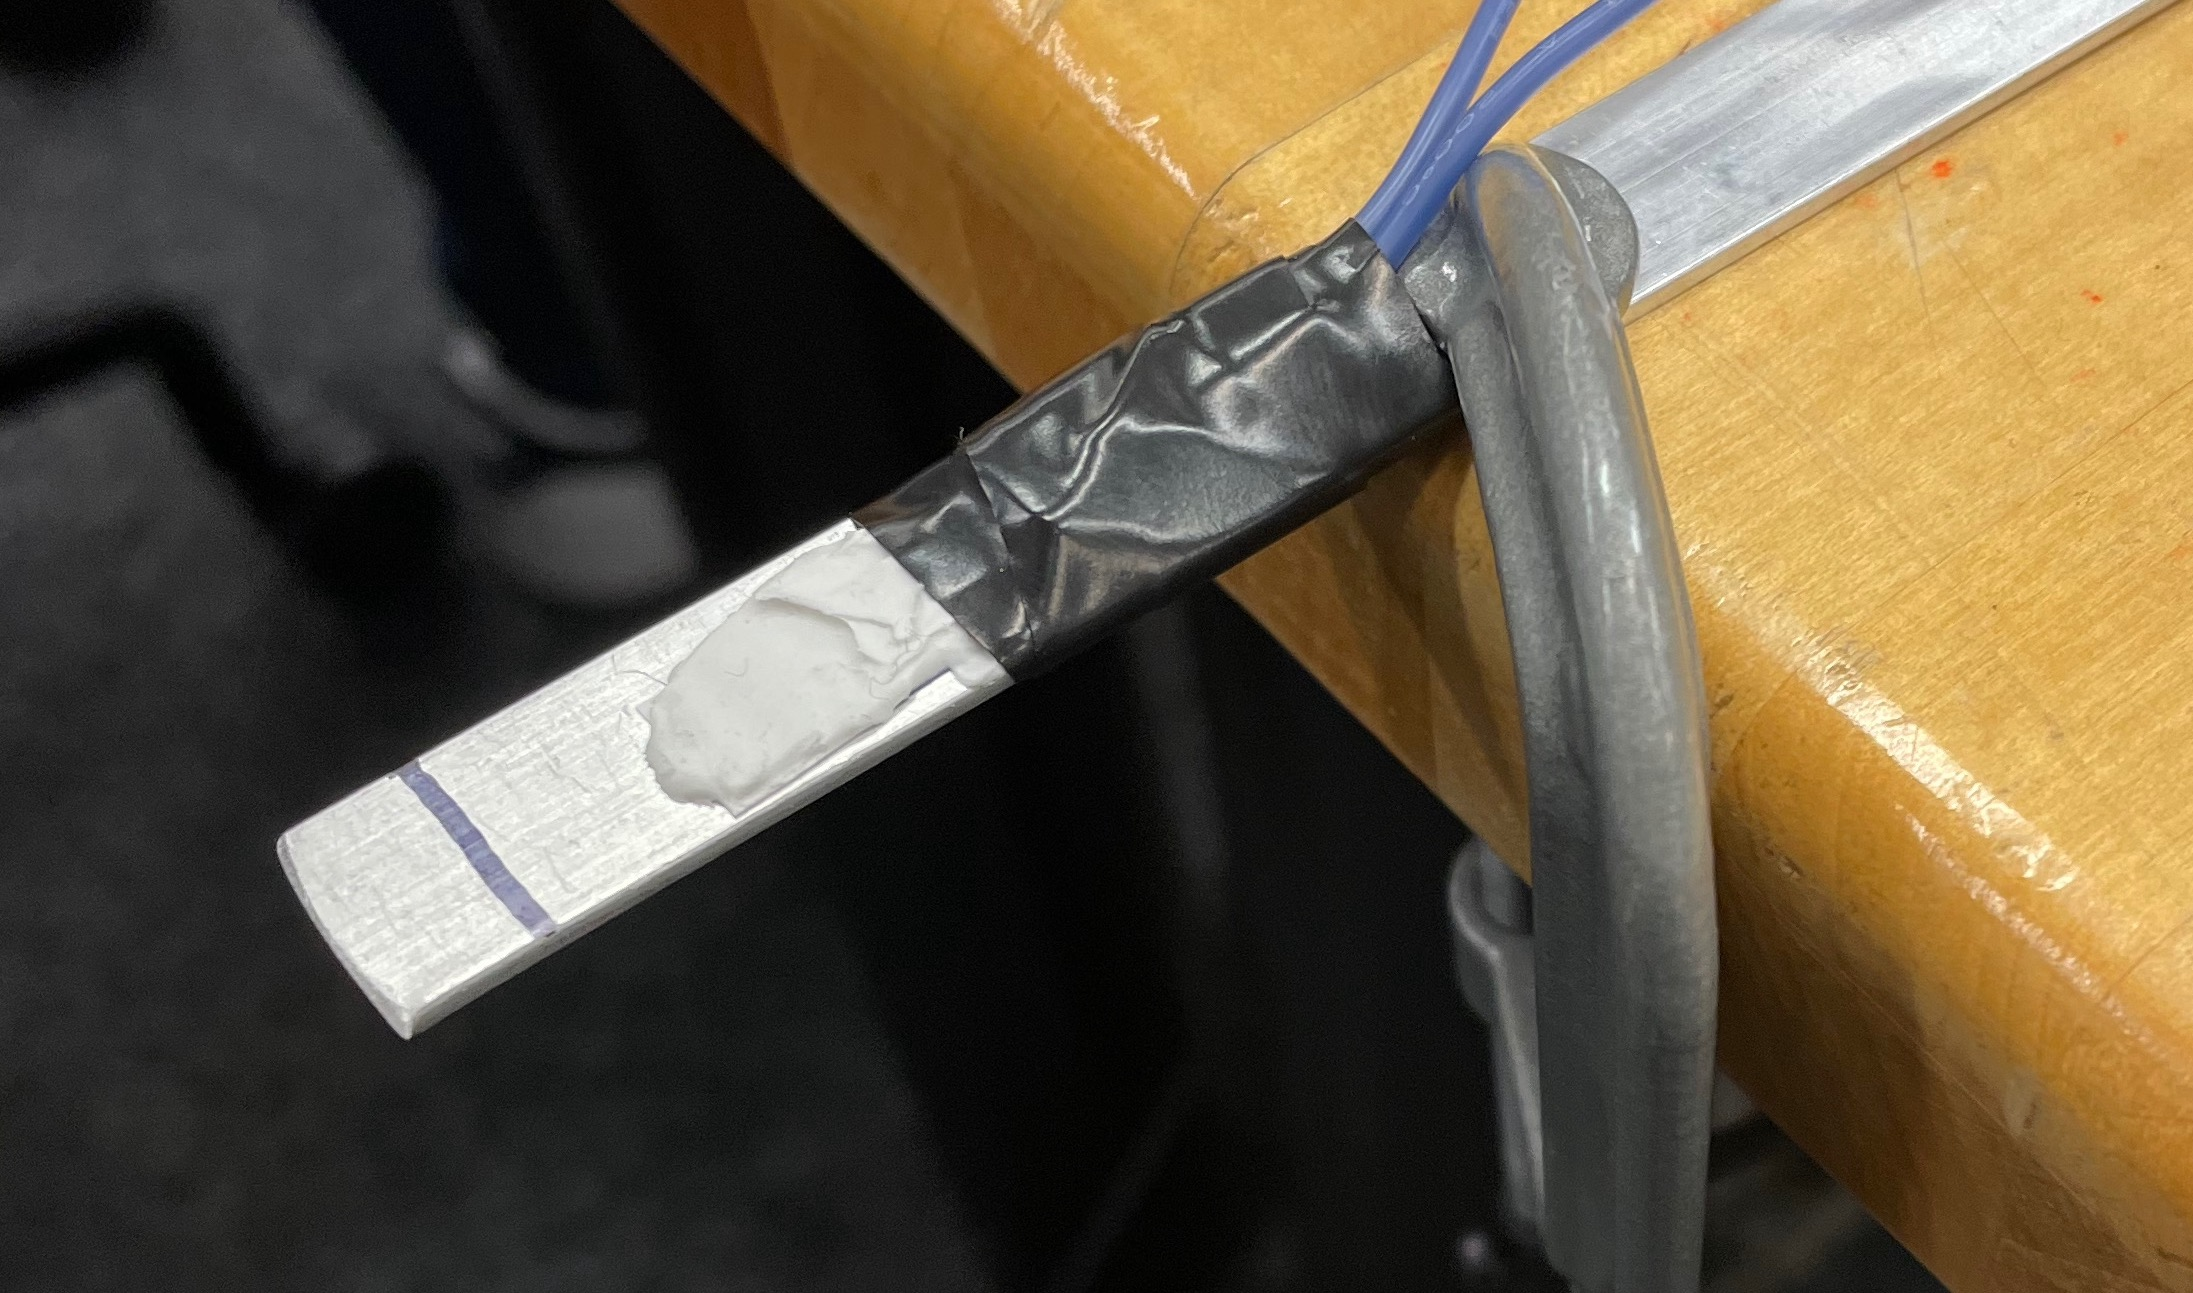
\includegraphics[width=0.5\textwidth]{strain_gauge.jpg}
	% here I put the width as a fraction of the text width. You can also use a set number of inches, mm, pt, etc.
	% the text in the curly brackets is the name of the file. If it doesn't work, try adding the file extension, e.g. .jpg
	
	\captionsetup{margin={0.28\textwidth,0.28\textwidth}}
	% by adding margins to your caption, you can make the caption wrap with your figures rather than at the normal text width
	
	\caption{\smaller{For this experiment, a strain gauge was laminated to an aluminum bar, then clamped to the edge of a table.}}
	% always caption your figures!
	
	\label{fig:strain_gauge}
	% the label here allows me to reference this figure in text anywhere in this document. By matching the text inside the curly brackets of \label{} here and \ref{} in a paragraph, LaTeX automatically inserts the correct figure number and creates a link between the number and the referenced figure. As good practice, always use "fig:" at the beginning of figure labels
\end{figure}

\subsection{Electronics}

In order to accurately measure small changes in the resistance of the strain gauge, we used a Wheatstone bridge, amplified using an AD623 IC and balanced using a $10 \Omega$ potentiometer (see Figure~\ref{fig:circuit}). An O-Scope was used to measure the voltage across the strain sensor from within the bridge (see Figure~\ref{fig:breadboard}).

\begin{figure} [!ht]
% the "!ht" will tell LaTeX to try and put the figure here, and at the top of the next page if it doesn't fit here. Getting figures to show up where you want can be a pain

	\centering  % this centers the image
	
	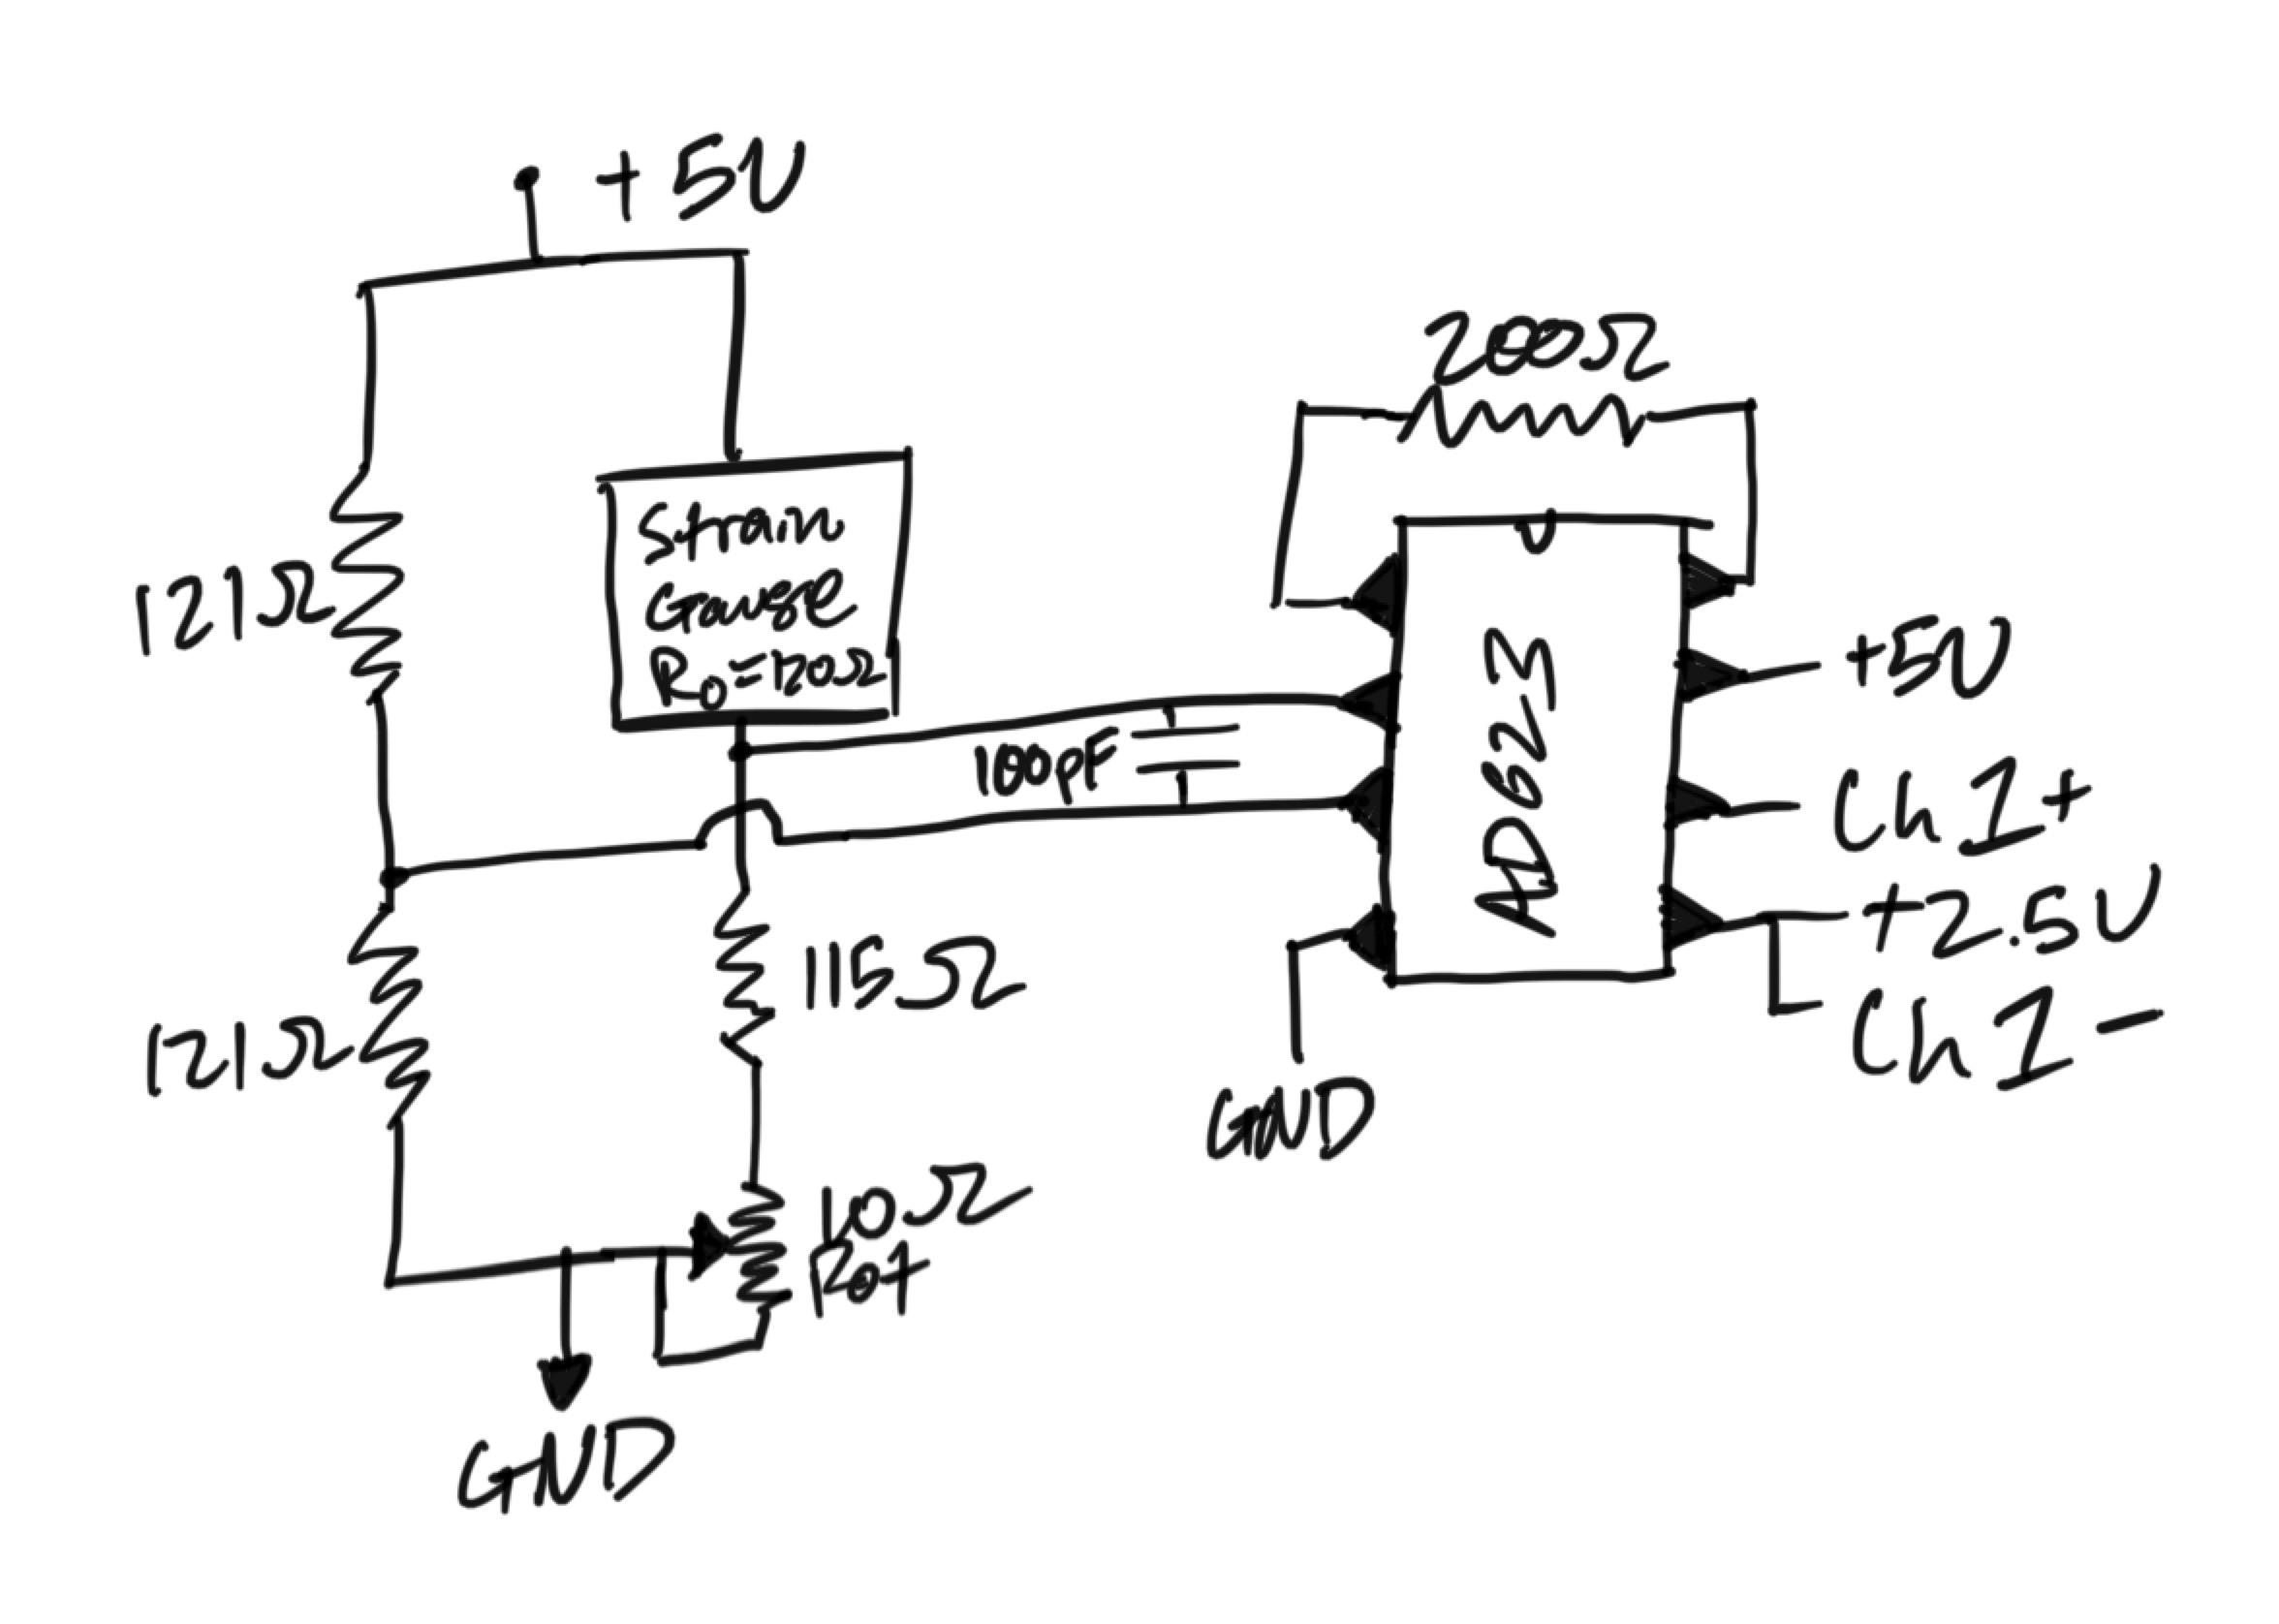
\includegraphics[width=0.75\textwidth]{circuit_diagram.jpg}
	% here I put the width as a fraction of the text width. You can also use a set number of inches, mm, pt, etc.
	% the text in the curly brackets is the name of the file. If it doesn't work, try adding the file extension, e.g. .jpg
	
	\captionsetup{margin={0.28\textwidth,0.28\textwidth}}
	% by adding margins to your caption, you can make the caption wrap with your figures rather than at the normal text width
	
	\caption{\smaller{We connected the strain gauge to an amplified Wheatstone bridge.}}
	% always caption your figures!
	
	\label{fig:circuit}
	% the label here allows me to reference this figure in text anywhere in this document. By matching the text inside the curly brackets of \label{} here and \ref{} in a paragraph, LaTeX automatically inserts the correct figure number and creates a link between the number and the referenced figure. As good practice, always use "fig:" at the beginning of figure labels
\end{figure}

\begin{figure} [!ht]
% the "!ht" will tell LaTeX to try and put the figure here, and at the top of the next page if it doesn't fit here. Getting figures to show up where you want can be a pain

	\centering  % this centers the image
	
	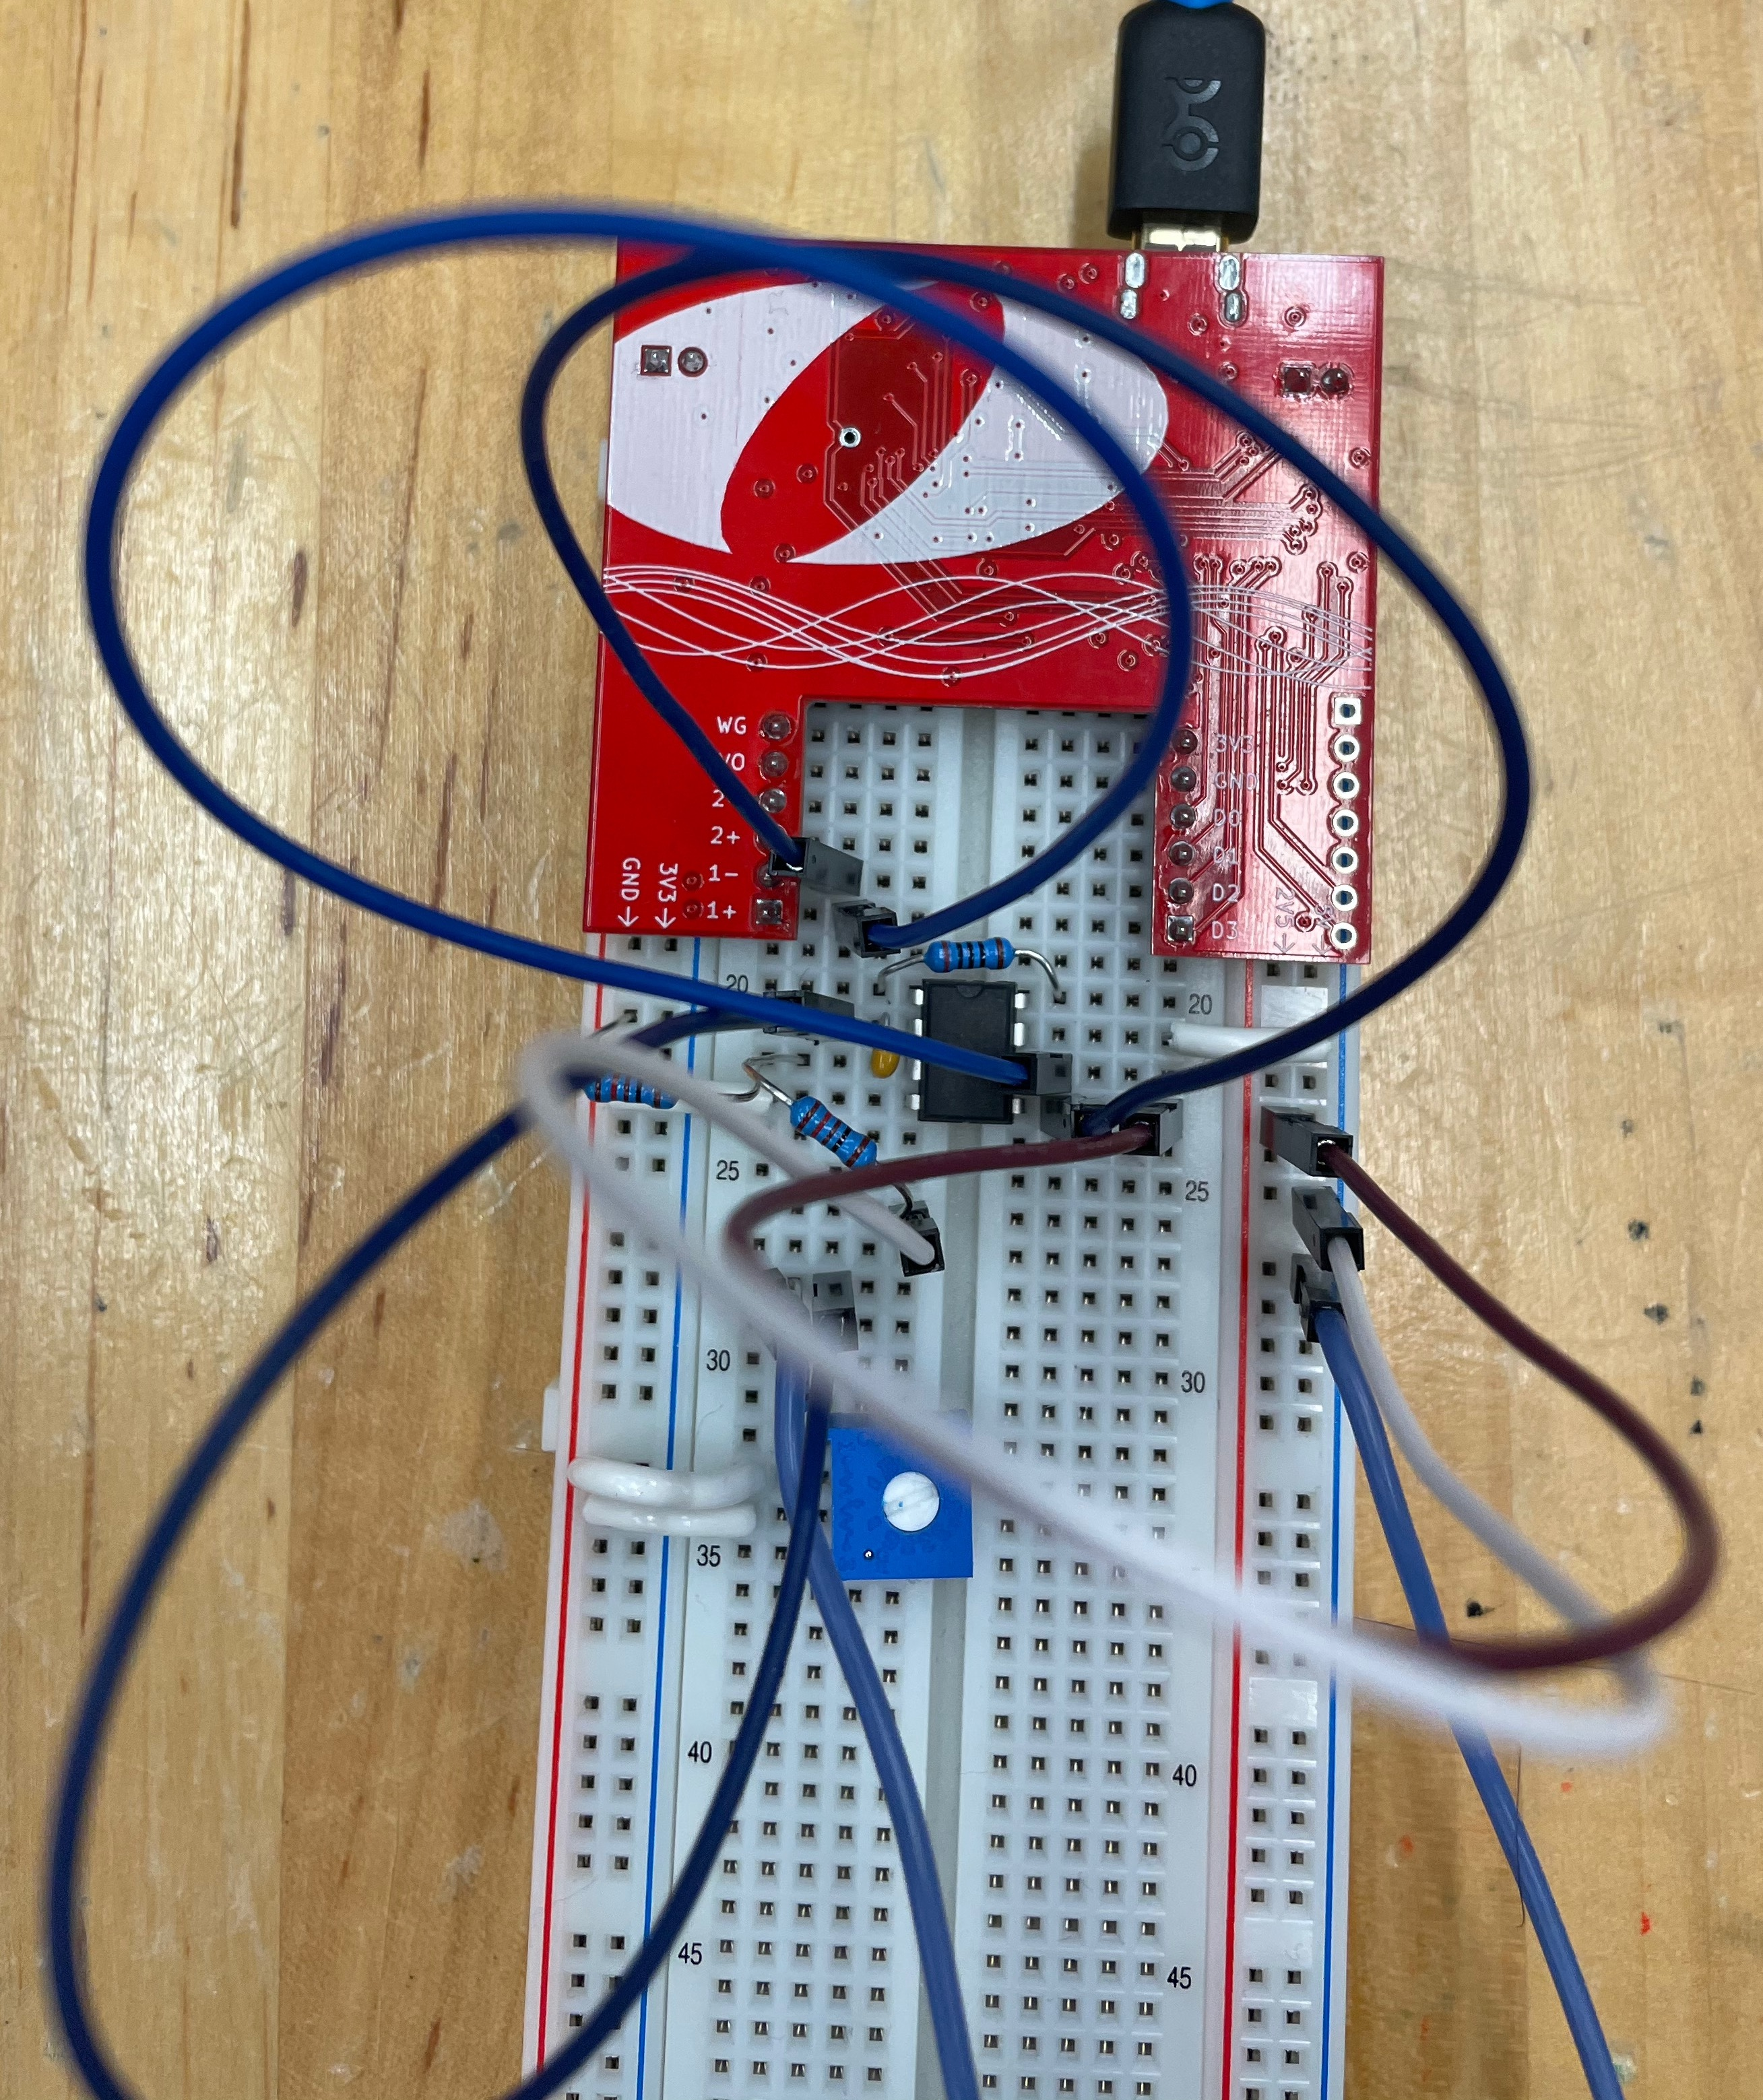
\includegraphics[width=0.5\textwidth]{breadboard.jpg}
	% here I put the width as a fraction of the text width. You can also use a set number of inches, mm, pt, etc.
	% the text in the curly brackets is the name of the file. If it doesn't work, try adding the file extension, e.g. .jpg
	
	\captionsetup{margin={0.28\textwidth,0.28\textwidth}}
	% by adding margins to your caption, you can make the caption wrap with your figures rather than at the normal text width
	
	\caption{\smaller{Our breadboard, as used to measure the voltage across the strain gauge using an amplified Wheatstone bridge.}}
	% always caption your figures!
	
	\label{fig:breadboard}
	% the label here allows me to reference this figure in text anywhere in this document. By matching the text inside the curly brackets of \label{} here and \ref{} in a paragraph, LaTeX automatically inserts the correct figure number and creates a link between the number and the referenced figure. As good practice, always use "fig:" at the beginning of figure labels
\end{figure}


\subsection{Calibration}

We knew that a strain sensor has a linear relationship between strain and resistance, which itself has a linear relationship to voltage. Additionally, an aluminum bar has a linear relationship between force applied (due to gravity) and strain. Consequently, we knew that there would be a linear relationship between the weight of an object hanging from the aluminum bar and the resistance of the strain gauge.

We determined this relationship by weighing three calibration objects, each with a known (but different) weight. For each object, we allowed the voltage reading to settle and then recorded the voltage measured by the O-Scope.

Finally, we computed a linear regression between measured voltage and known weight. This regression allowed us to calculate the measured weight from an arbitrary voltage across the strain sensor.

\subsection{Testing}

As the last step in our experiment, we weighed a fourth and object of known weight, which had not yet been weighed by our strain gauge scale. We used the calculated linear regression to determine the measured weight of the object, and compared that to known weight to calculate the error.

\section{Results}

\subsection{Calibration}

We calibrated our scale using three objects, with the following known weights and measured voltages:

\begin{table}[!ht]
    \centering
    \begin{tabular}{ll}
    \hline
    \multicolumn{1}{c}{\textbf{Measured Voltage (mV)}} & \multicolumn{1}{c}{\textbf{Known Weight (g)}} \\ \hline
    9mV                                                & 14g                                           \\
    30mV                                               & 27.7g                                         \\
    45mV                                               & 40.7g                                         \\ \hline
    \end{tabular}
    \caption{\smaller{Measured voltages and known weights of our three calibration objects.}}
    \label{table:calibration}
\end{table}

From this data, we calculated the following linear regression, which represents our scale's relationship between voltage ($V$) and mass ($m$). A visual comparison between our data and the regression can also be seen in Figure~\ref{fig:calibration}.

\begin{equation}
    \text{m} = 1.35V - 9.0792
\end{equation}

\begin{figure}[!ht]
	\centering 
	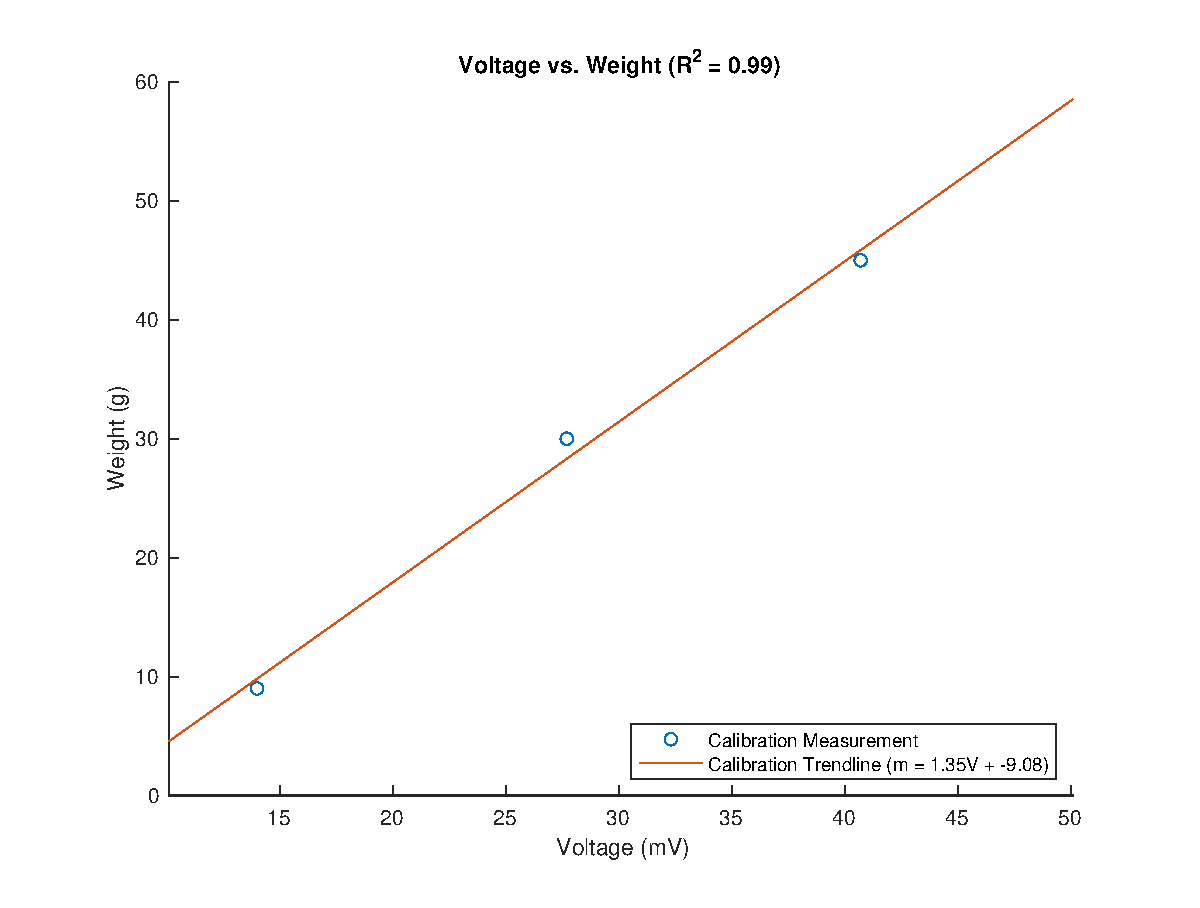
\includegraphics[width=0.7\textwidth]{calibration.eps}
	\captionsetup{margin={0.2\textwidth,0.2\textwidth}}
	\caption{\smaller{Voltage vs. weight, showing our three calibration weights and our calculated calibration trendline. $R^2 = 0.99$}}
	\label{fig:calibration}
\end{figure}

\subsection{Testing}

After calculating our trendline, we weighed another test object, measured the voltage across the strain gauge, and calculated the measured weight of the object. The object's true weight was 57.1g while its measured weight was 59.77g (see Figure~\ref{fig:weights}, for an error of 4.67\%. That error is fairly low, making our strain gauge a decent means of weight measurement.

\begin{figure}[!ht]
	\centering 
	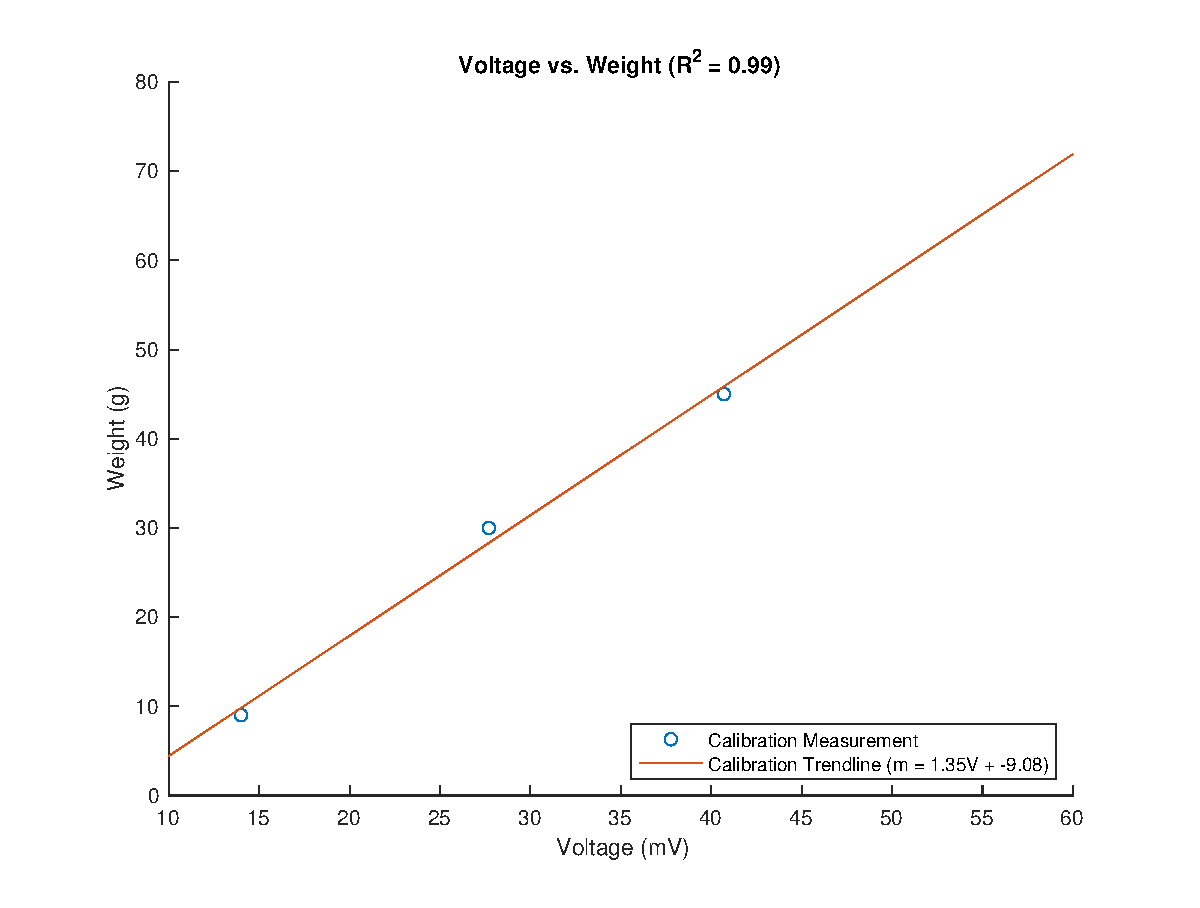
\includegraphics[width=0.7\textwidth]{weights.eps}
	\captionsetup{margin={0.2\textwidth,0.2\textwidth}}
	\caption{\smaller{Voltage vs. weight, showing the test object's measured and true weight in addition to our three calibration weights and our calculated calibration trendline.}}
	\label{fig:weights}
\end{figure}

\subsection{Sensitivity}

The sensitivity of our strain gauge was $0.74\frac{mV}{g}$. Assuming that a $5mV$ change is easily detectable by our equipment, the resolution of our scale is $6.76g$, which is a reasonable level of precision for many tasks.

For our system, a $20mV$ change in output voltage represents an additional $27.03g$ of weight added to the scale, as calculated by our linear regression. It also corresponds to a $1.48\Omega$ change in the electrical resistance of the strain gauge, as calculated from the formulae given by the ISIM teaching team for voltage dividers, the strain gauge resistance/deformation relationship, and the AD632 input/output relationship.

\section{Finishing Remarks}
This experiment demonstrated that an electric strain gauge has significant potential a mechanism for measuring weight. More experimentation is required to determine how to reduce noise and increase precision.
\end{document}